\chapter{Specyfikacja}

\section{Wymagania funkcjonalne}

\begin{table}[H]
    \begin{tabular}{|p{5cm}|p{9cm}|}\hline
    ID: & UC00 \\ \hline
    Nazwa: & Dodawanie przedmiotu \\\hline
    Aktorzy: & Użytkownik zalogwany, System \\\hline
    Poziom: & Poziom użytkownika  \\\hline
    Priorytet: & Wysoki \\\hline
    Warunki początkowe: & ~ \\\hline
    Scenariusz główny: & 1. Użytkownik wybiera opcję dodania produktu do bazy danych systemu. \\
    ~ & 2. System prosi recenzenta o podanie wymaganych informacji o produkcie. \\
    ~ & 3. Recenzent podaje wszystkie obowiązkowe dane. \\
    ~ & 4. Recenzent zatwierdza informacje. \\
    ~ & 5. System dodaje produkt do bazy danych. \\\hline
    Scenariusz alternatywny & 3a. Kategoria przedmiotu nie istnieje w systemie: \\
    i rozszerzenia: & 3a.1. Użytkownik wybiera opcję dodania nowej kategorii. \\
    ~ & 3a.2. Przejdź do UC04. \\
    ~ & 3a.3. Powrót do punktu 3. \\
    ~ & 4a. Podane dane są nieprawidłowe: \\
    ~ & 4a.1. System prosi o poprawienie błędnych danych. \\
    ~ & 4a.2. Recenzent wprowadza poprawne dane. \\
    ~ & 4a.3. Powrót do punktu 4. \\
    \hline\end{tabular}
\end{table}

\begin{table}[H]
    \begin{tabular}{|p{5cm}|p{9cm}|}\hline
	ID: & UC01  \\\hline
    Nazwa: & Dodawanie recenzji \\\hline
    Aktorzy: & Recenzent, System \\\hline
    Poziom: & Poziom użytkownika  \\\hline
    Priorytet: & Wysoki \\\hline
    Warunki początkowe: & ~ \\\hline
    Scenariusz główny: & 1. Recenzent przechodzi na stronę produktu, którego recenzję chce dodać. \\
    ~ & 2. Recenzent wybiera opcję dodania recenzji produktu. \\
    ~ & 3. System prezentuje Recenzentowi ekran dodawania recenzji. \\
    ~ & 4. Recenzent wypełnia formularz dodawania recenzji. \\
    ~ & 5. Recenzent potwierdza chęć dodania recenzji. \\
    ~ & 6. System publikuje recenzję w serwisie. \\
    ~ & ~ \\\hline
    Scenariusz alternatywny & 1a. Szukany produkt nie istnieje: \\
    i rozszerzenia: & 1a.1. Przejdź do UC00. \\
    ~ & 1a.2. Powrót do punktu 1. \\
    ~ & 2a. Użytkownik jest niezalogowany: \\
    ~ & 2a.1. Przejdź do UC02. \\
    ~ & 2a.2. Przejdź do punktu 3. \\
    ~ & 5a. Formularz wypełniono nieprawidłowo (np. nie wypełniono wszystkich obowiązkowych pól): \\
    ~ & 5a.1. System prosi o poprawienie błędnych danych. \\
    ~ & 5a.2. Recenzent wprowadza poprawne dane. \\
    ~ & 5a.3. Przejdź do punktu 5. \\
    \hline\end{tabular}
\end{table}

\begin{table}[H]
    \begin{tabular}{|p{5cm}|p{9cm}|}\hline
    ID: & UC02 \\\hline
    Nazwa: & Logowanie do serwisu \\\hline
    Aktorzy: & System, Użytkownik niezalogowany \\\hline
    Poziom: & Poziom użytkownika  \\\hline
    Priorytet: & Wysoki \\\hline
    Warunki początkowe: & ~ \\\hline
    Scenariusz główny: & 1. System prezentuje formularz logowania \\
    ~ & 2. Użytkownik wprowadza swoje dane \\
    ~ & 3. System dokonuje uwierzytelnienia użytkownika \\ \hline
    Scenariusz alternatywny & 2a. Podane dane są niepoprawne \\
    i rozszerzenia: & 2a.1. System informuje o błędnych danych logowania \\
    ~ & 2a.2. Powrót do punktu 1 \\
    ~ & 2b. Użytkownik nie posiada konta w systemie \\
    ~ & 2b.1. Przejdź do UC03. \\
    ~ & 2b.2. Powrót do punktu 1.  \\
    \hline\end{tabular}
\end{table}

\begin{table}[H]
    \begin{tabular}{|p{5cm}|p{9cm}|}\hline
    ID: & UC03 \\\hline
    Nazwa: & Rejestracja w serwisie \\\hline
    Aktorzy: & System, Użytkownik niezalogowany \\\hline
    Poziom: & Poziom użytkownika  \\\hline
    Priorytet: & Wysoki \\\hline
    Warunki początkowe: & ~ \\\hline
    Scenariusz główny: & 1. System prezentuje formularz rejestracji \\
    ~ & 2. Użytkownik wprowadza swoje dane \\
    ~ & 3. System tworzy konto Użytkownika \\\hline
    Scenariusz alternatywny & 2a. Podane dane są niepoprawne \\
    i rozszerzenia: & 2a.1. System informuje o błędnych danych rejestracyjnych \\
    ~ & 2a.2. Powrót do punktu 1 \\
    \hline\end{tabular}
\end{table}
\newpage
\begin{table}[H]
    \begin{tabular}{|p{5cm}|p{9cm}|}\hline
	ID: & UC04 \\\hline
    Nazwa: & Dodawanie kategorii \\\hline
    Aktorzy: & Użytkownik zalogowany, System \\\hline
    Poziom: & Poziom użytkownika  \\\hline
    Priorytet: & Średni \\\hline
    Warunki początkowe: & ~ \\\hline
    Scenariusz główny: & 1. System prezentuje ekran z formularzem dodawania kategorii \\
    ~ & 2. System prosi Użytkownika o podanie wymaganych informacji o kategorii \\
    ~ & 3. Użytkownik podaje wszystkie obowiązkowe dane \\
    ~ & 4. Użytkownik zatwierdza operację \\
    ~ & 5. System dodaje kategorię \\\hline
    Scenariusz alternatywny & 4a. Podane dane są nieprawidłowe \\
    i rozszerzenia: & 4a.1. System prosi o poprawienie błędnych danych \\
    ~ & 4a.2. Użytkownik wprowadza poprawne dane. \\
    ~ & 4a.4. Powrót do punktu 4 \\
    \hline\end{tabular}
\end{table}

\begin{table}[H]
    \begin{tabular}{|p{5cm}|p{9cm}|}\hline
    ID: & UC05 \\\hline
    Nazwa: & Przeglądanie profilu recenzenta \\\hline
    Aktorzy: & System, Użytkownik \\\hline
    Poziom: & Poziom użytkownika  \\\hline
    Priorytet: & Niski \\\hline
    Warunki początkowe: & ~ \\\hline
    Scenariusz główny: & 1. Użytkownik wybiera opcję wyświetlenia profilu danego recenzenta (w tym swojego) \\
    ~ & 2. System prezentuje ekran profilu, wyświetlając informacje o Recenzencie oraz listę jego recenzji \\\hline
    Scenariusz alternatywny & ~ \\
	i rozszerzenia: & ~ \\
    \hline\end{tabular}
\end{table}
\newpage
\begin{table}[H]
    \begin{tabular}{|p{5cm}|p{9cm}|}\hline
    ID: & UC06 \\\hline
    Nazwa: & Przeglądanie listy recenzji produktu \\\hline
    Aktorzy: & System, Użytkownik \\\hline
    Poziom: & Poziom użytkownika  \\\hline
    Priorytet: & Wysoki \\\hline
    Warunki początkowe: & ~ \\\hline
    Scenariusz główny: & 1. System wyświetla listę wszystkich recenzji dotyczących wybranego produktu \\
    ~ & 2. Użytkownik wybiera interesującą go recenzję \\
    ~ & 3. System wyświetla wybraną recenzję (UC08) \\\hline
    Scenariusz alternatywny & ~ \\
	i rozszerzenia: & ~ \\
    \hline\end{tabular}
\end{table}

\begin{table}[H]
    \begin{tabular}{|p{5cm}|p{9cm}|}\hline
    ID: & UC07 \\\hline
    Nazwa: & Przeglądanie produktów \\\hline
    Aktorzy: & System, Użytkownik \\\hline
    Poziom: & Poziom użytkownika  \\\hline
    Priorytet: & Wysoki \\\hline
    Warunki początkowe: & ~ \\\hline
    Scenariusz główny: & 1. System wyświetla listę najnowszych recenzji i produktów \\
    ~ & 2. Użytkownik wpisuje pożądane wartości flitrów, wg których chce ograniczyć listę produktów (nazwę produktu lub jego parametry) \\
    ~ & 3. System zastępuje listę najnowszych pozycji listą produktów dopasowanych do kryteriów wyszukiwania \\
    ~ & 4. Użytkownik wybiera konkretny produkt \\
    ~ & 5. System prezentuje listę recenzji wybranego produktu (UC06) \\\hline
    Scenariusz alternatywny & 2a. Użytkownik nie wpisuje żadnego ograniczenia \\
    i rozszerzenia: & 2a.1. Użytkownik wybiera jedną z przedstawionych najnowszych pozycji (UC06 lub UC08) \\
	\hline\end{tabular}
\end{table}
\newpage
\begin{table}[H]
    \begin{tabular}{|p{5cm}|p{9cm}|}\hline
    ID: & UC08 \\\hline
    Nazwa: & Przeglądanie konkretnej recenzji \\\hline
    Aktorzy: & System, Użytkownik \\\hline
    Poziom: & Poziom użytkownika  \\\hline
    Priorytet: & Wysoki \\\hline
    Warunki początkowe: & ~ \\\hline
    Scenariusz główny: & 1. System prezentuje ekran konkretnej recenzji, z jej treścią, oceną końcową oraz komentarzami do recenzji \\
    ~ & 2. Użytkownik ocenia przydatność recenzji poprzez kliknięcie odpowiedniego przycisku \\
    ~ & 3. Użytkownik przegląda komentarze do recenzji \\\hline
    Scenariusz alternatywny & 2a. Użytkownik nie ocenia przydatności recenzji \\
    i rozszerzenia: & 3a. Użytkownik dodaje własny komentarz \\
    ~ & 3b. Użytkownik oznacza istniejący komentarz jako spam \\
    \hline\end{tabular}
\end{table}

\begin{table}[H]
    \begin{tabular}{|p{5cm}|p{9cm}|}\hline
    ID: & UC09 \\\hline
    Nazwa: & Subskrybcja produktu \\\hline
    Aktorzy: & System, Użytkownik zalogowany \\\hline
    Poziom: & Poziom użytkownika  \\\hline
    Priorytet: & Niski \\\hline
    Warunki początkowe: & ~ \\\hline
    Scenariusz główny: & 1. Użytkownik wchodzi na stronę ekran konkretnego produktu \\
    ~ & 2. Użytkownik wybiera opcję zasubskrybowania tego produktu \\
    ~ & 3. System okresowo wysyła użytkownikowi informacje o nowych recenzjach tego produktu \\\hline
    Scenariusz alternatywny & 2a. Użytkownik nie jest zalogowany \\
    i rozszerzenia: & 2a.1. System prosi o zalogowanie (UC02) \\
    ~ & 2a.2. Powrót do punktu 2  \\
    \hline\end{tabular}
\end{table}
\newpage
\begin{table}[H]
    \begin{tabular}{|p{5cm}|p{9cm}|}\hline
    ID: & UC10 \\\hline
    Nazwa: & Subskrypcja recenzenta \\\hline
    Aktorzy: & System, Użytkownik zalogowany \\\hline
    Poziom: & Poziom użytkownika  \\\hline
    Priorytet: & Niski \\\hline
    Warunki początkowe: & ~ \\\hline
    Scenariusz główny: & 1. Użytkownik wchodzi na stronę ekran profilu recenzenta \\
    ~ & 2. Użytkownik wybiera opcję zasubskrybowania tego recenzenta \\
    ~ & 3. System okresowo wysyła użytkownikowi informacje o nowych recenzjach tego recenzenta \\\hline
    Scenariusz alternatywny & 2a. Użytkownik nie jest zalogowany \\
    i rozszerzenia: & 2a.1. System prosi o zalogowanie (UC02) \\
    ~ & 2a.2. Powrót do punktu 2  \\
    \hline\end{tabular}
\end{table}

\begin{table}[H]
    \begin{tabular}{|p{5cm}|p{9cm}|}\hline
    ID: & UC11 \\\hline
    Nazwa: & Wyszukiwanie produktu \\\hline
    Aktorzy: & System, Użytkownik \\\hline
    Poziom: & Poziom użytkownika  \\\hline
    Priorytet: & Średni \\\hline
    Warunki początkowe: & ~ \\\hline
    Scenariusz główny: & 1. Użytkownik wpisuje frazę wyszukiwania do odpowiedniego pola \\
    ~ & 2. System prezentuje listę znalezionych produktów \\
    ~ & 3. Użytkownik wybiera interesujący go produkt \\\hline
	Scenariusz alternatywny & ~ \\
	i rozszerzenia: & ~ \\
    \hline\end{tabular}
\end{table}
\newpage
\begin{table}[H]
    \begin{tabular}{|p{5cm}|p{9cm}|}\hline
    ID: & UC12 \\\hline
    Nazwa: & Przeglądanie subskrybcji \\\hline
    Aktorzy: & System, Użytkownik zalogowany \\\hline
    Poziom: & Poziom użytkownika  \\\hline
    Priorytet: & Niski \\\hline
    Warunki początkowe: & ~ \\\hline
    Scenariusz główny: & 1. Użytkownik wchodzi na ekran profilu \\
    ~ & 2. Użytkownik wybiera opcję wyświetlenia sybskrybcji \\
    ~ & 3. System wyświetla listę atywnych subskrybcji użytkownika \\\hline
    Scenariusz alternatywny i~rozszerzenia:& 3a. Użytkownik wybiera opcję rezygnacji ze wskazanej subskrybcji \\
    ~ & 3a.1. System anuluje wybraną subskrypcję \\
    \hline\end{tabular}
\end{table}

\section{Wymagania pozafunkcjonalne}
\begin{itemize}
\item System powinien działać prawidłowo na przeglądarkach Chrome, Opera, Safari, Firefox oraz Internet Explorer
\item Dane w systemie powinny być przechowywane w grafowej bazie danych
\item Kod źródlowy powinien być stworzony zgodnie ze standardami wybranego języka
\item Maksymalny czas odpowiedzi systemu powinien być mniejszy niż 3 sek.
\item Hasła użytkowników powinny być przechowywane w postaci zaszyfrowanej
\item System powinien uniemożliwiać łatwe podszycie się pod innego użytkownika 
\item Dane powinny być pobierane do systemu za pośrednictwem zewnętrznego API
\item Źródło danych powinno być w łatwy sposób podmienialne
\item System powinien posiadać modularną strukturę, pozwalającą na łatwą podmianę np. frontendu
\end{itemize}

\section{Aktorzy i charakterystyka użytkowników}
\begin{figure}[H]
	\centering
	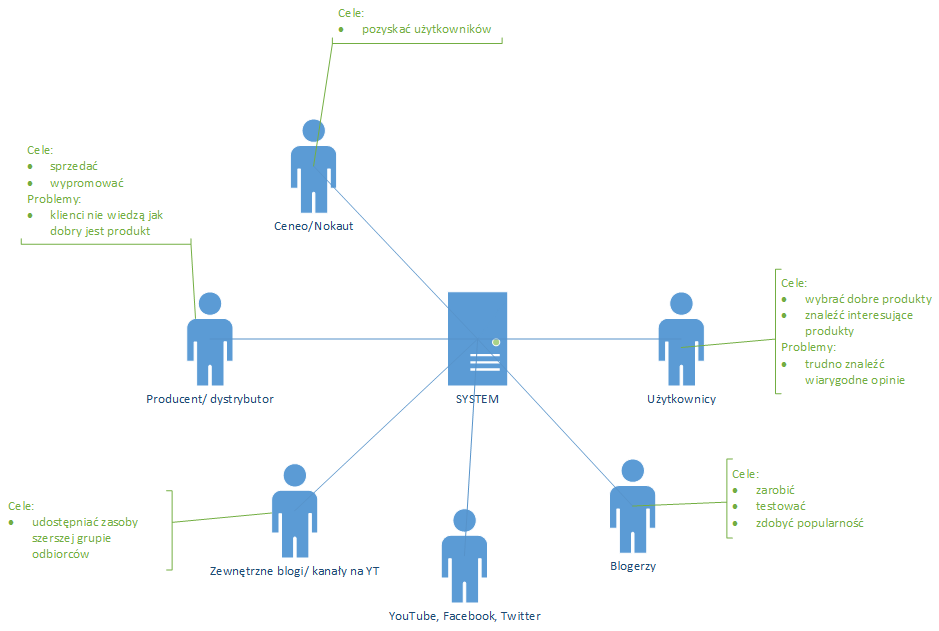
\includegraphics[width=\textwidth, keepaspectratio=true]{images/Strony_cele.png}
	\caption{Aktorzy i charakterystyka użytkowników}
\end{figure}
\section{Struktura programowa}
\begin{figure}[H]
	\centering
	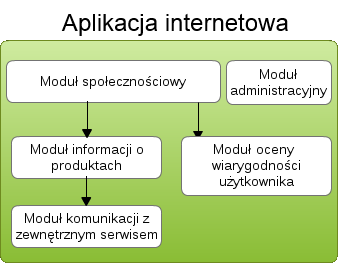
\includegraphics[scale=0.9]{images/modules.png}
	\caption{Struktura programowa}
\end{figure}
\section{Architektura systemu}
\begin{figure}[H]
	\centering
	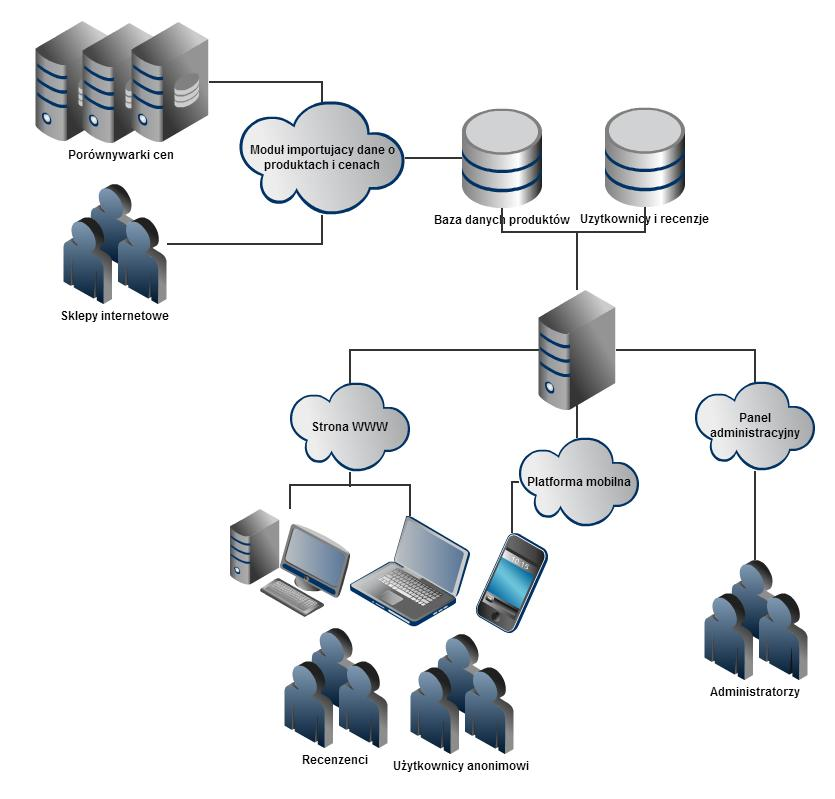
\includegraphics[scale=0.5]{images/architektura.jpg}
	\caption{Architektura systemu}
\end{figure}
\newpage
\section{Warstwy implementacyjne}
\begin{figure}[H]
	\centering
	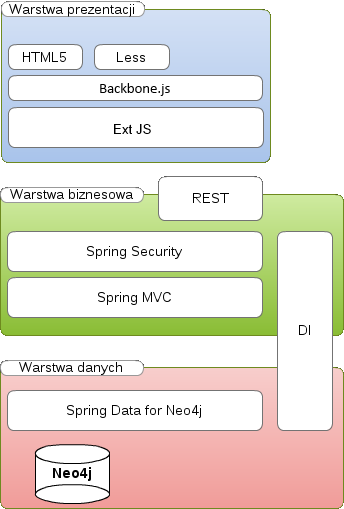
\includegraphics[scale=0.9]{images/warstwy.png}
	\caption{Warstwy implementacyjne}
\end{figure}


